
	\begin{frame}[c]\frametitle{Another Problem}
		\begin{columns}
			\column{4cm}
			\begin{itemize}
				\item<1-> an undirected graph
				\item<2-> add $x$ to $u$
				\item<5-> query neighbors' sum
				\item<7-> $O(m)=n$
			\end{itemize}
			\column{6cm}
			\only{\centering{{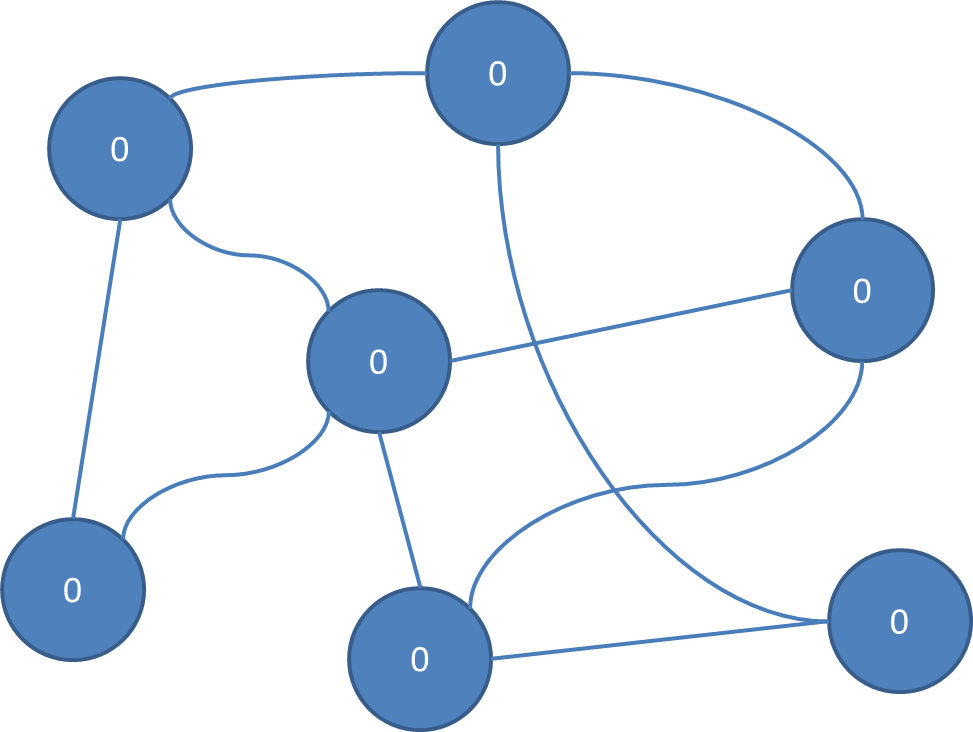
\includegraphics[width=6cm]{qwd_part/0.png}<1>}}}
			\only{\centering{{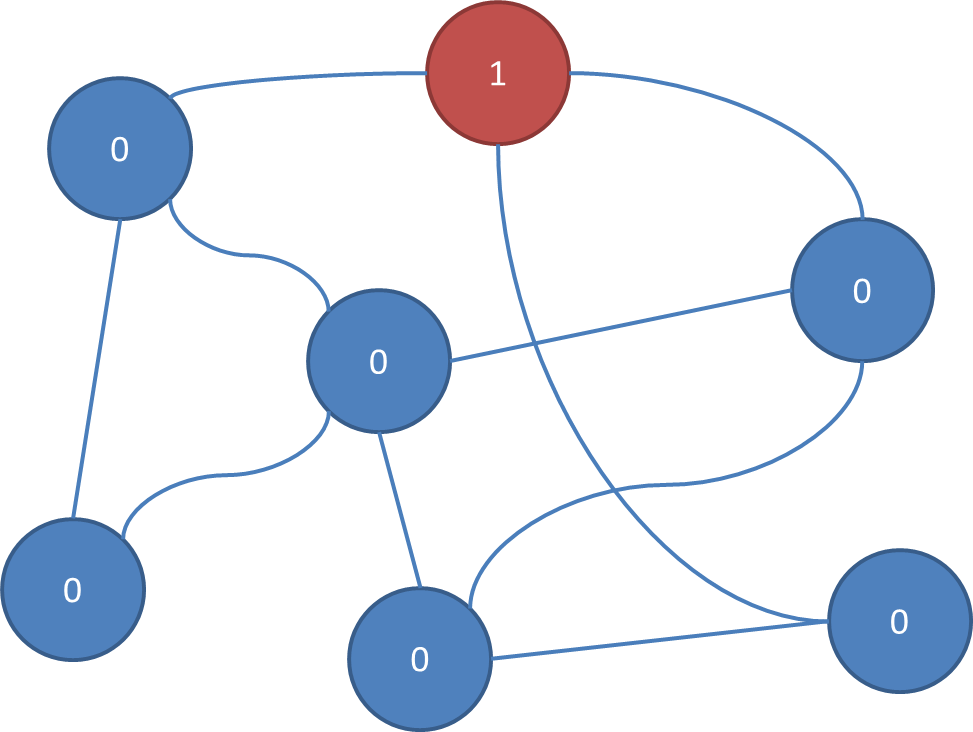
\includegraphics[width=6cm]{qwd_part/1.png}<2>}}}
			\only{\centering{{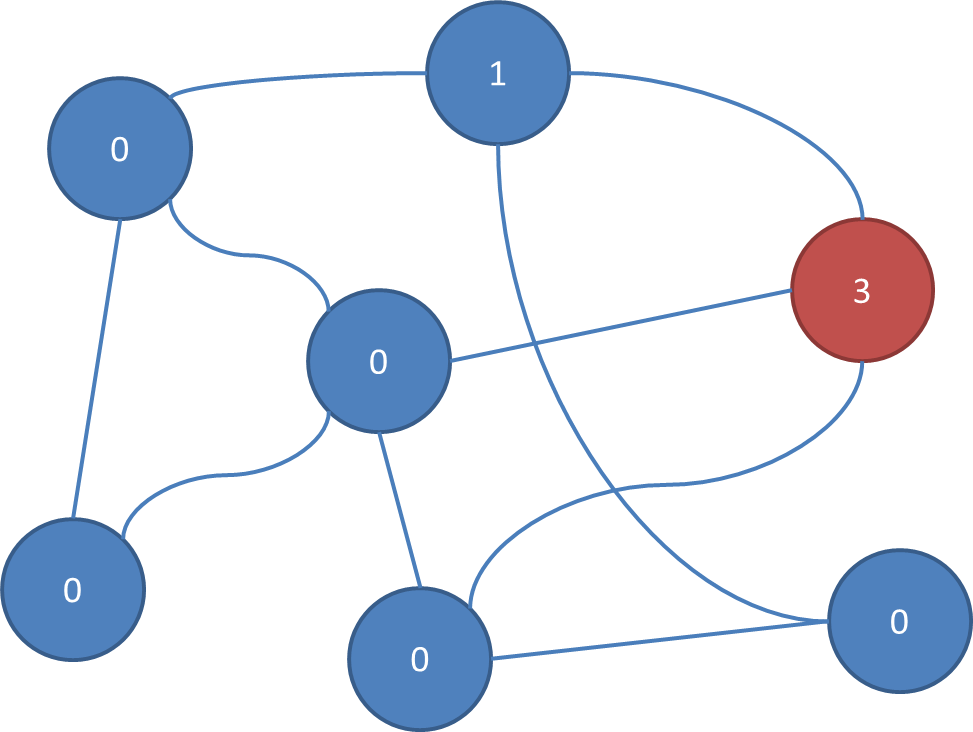
\includegraphics[width=6cm]{qwd_part/2.png}<3>}}}
			\only{\centering{{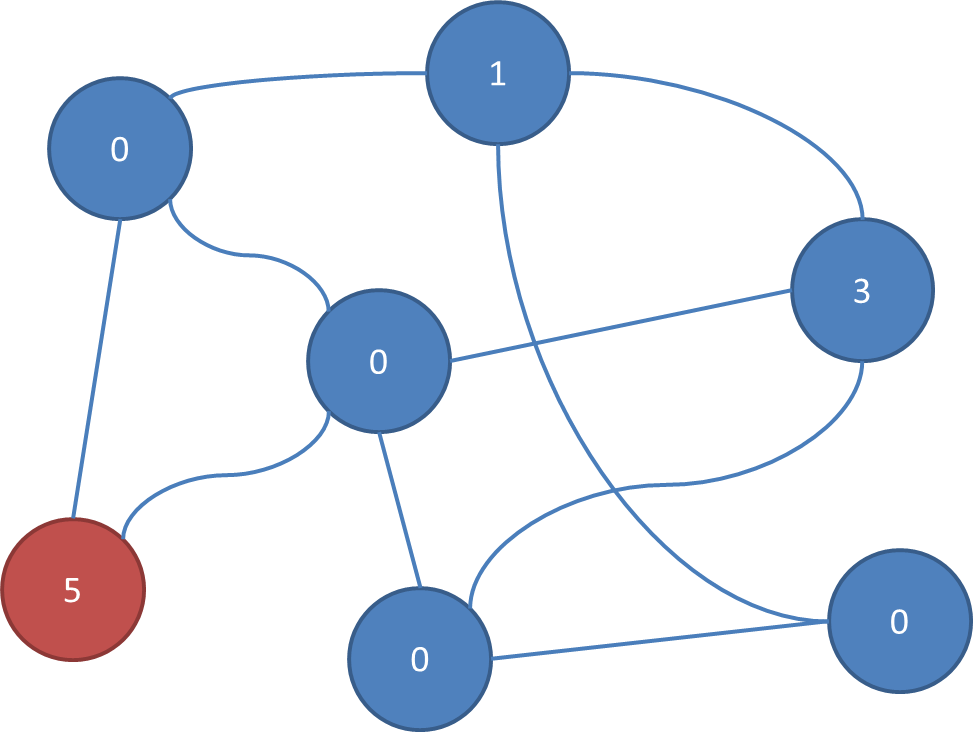
\includegraphics[width=6cm]{qwd_part/3.png}<4>}}}
			\only{\centering{{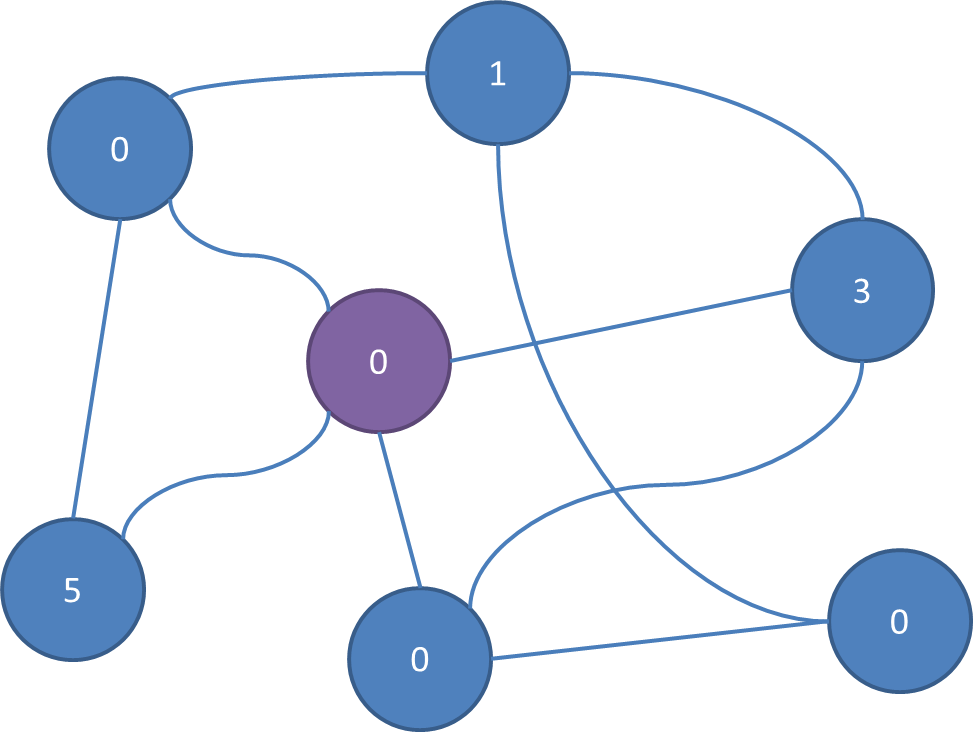
\includegraphics[width=6cm]{qwd_part/5.png}<5>}}}
			\only{\centering{{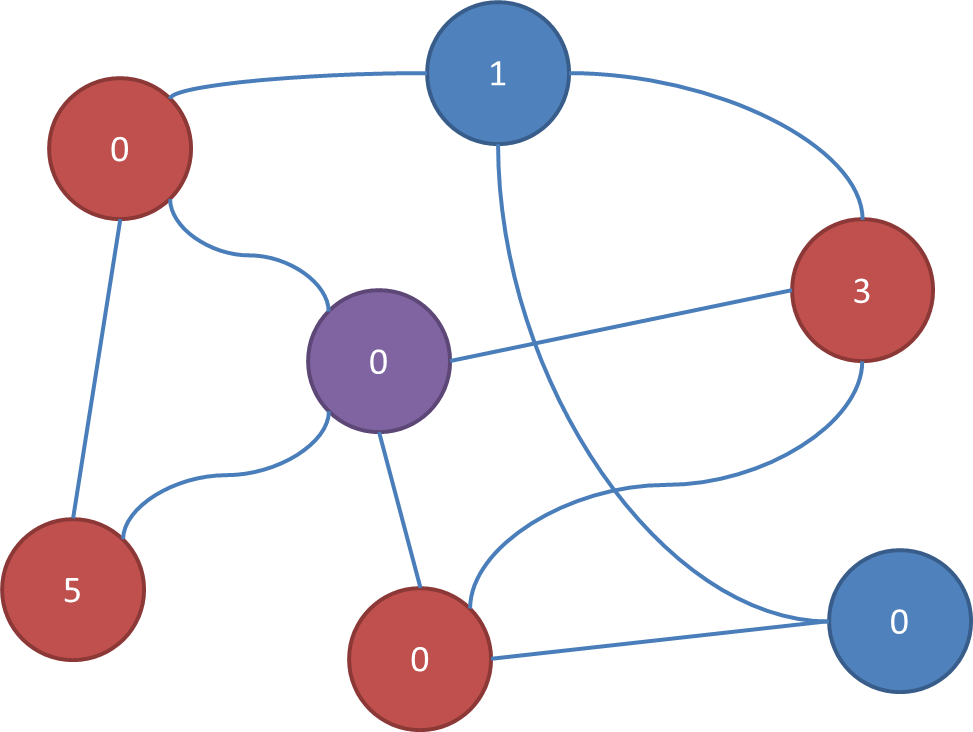
\includegraphics[width=6cm]{qwd_part/6.png}<6>}}}
			\only{\centering{{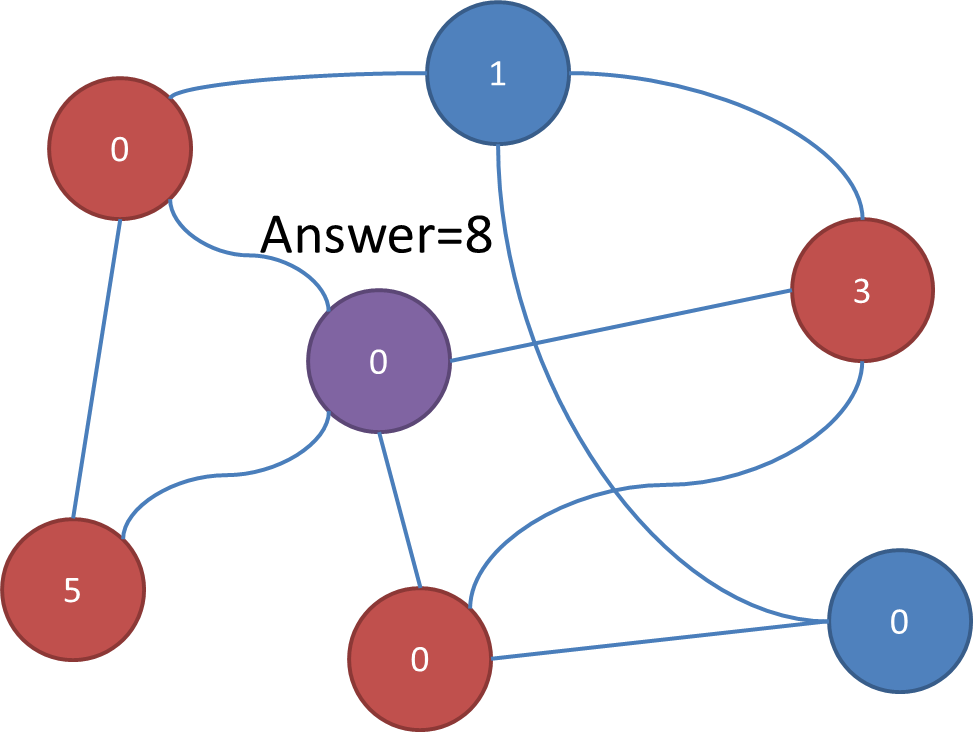
\includegraphics[width=6cm]{qwd_part/7.png}<7>}}}
		\end{columns}
	\end{frame}
	\begin{frame}[c]\frametitle{Naive Approach 1}
		\begin{columns}
			\column{4cm}
			\beamerdefaultoverlayspecification{<+->}
			\begin{itemize}
				\item store the value $v[x]$
				\item $O(n)$ space
				\item $O(1)$ time for add
				\item $O(n)$ time for query
			\end{itemize}
			\column{6cm}
			\only{\centering{{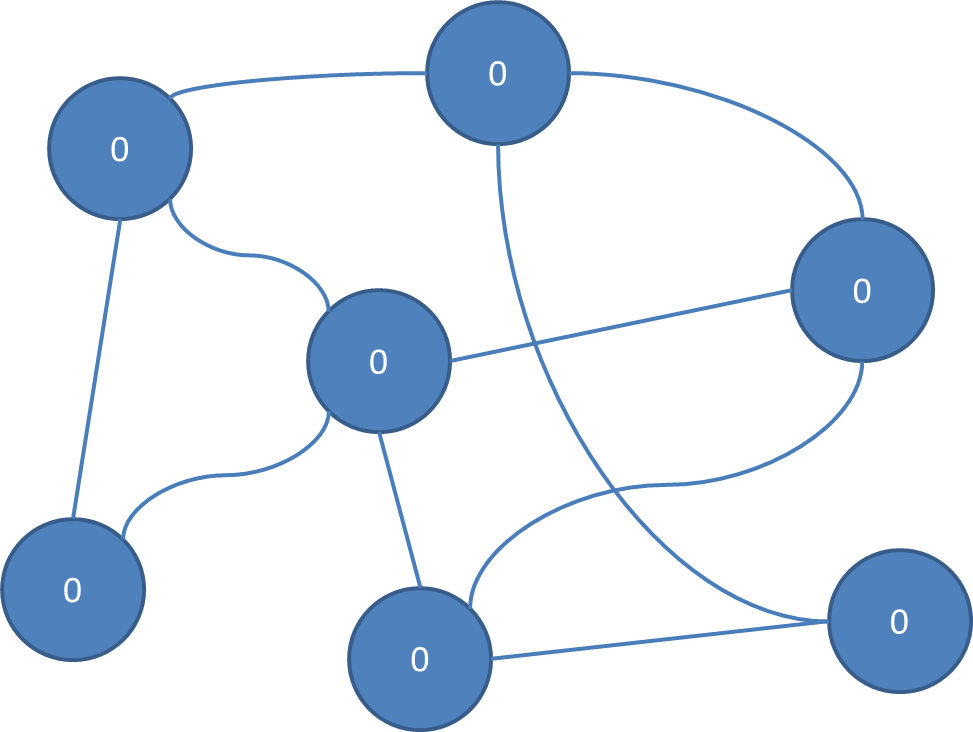
\includegraphics[width=6cm]{qwd_part/0.png}<1-2>}}}
			\only{\centering{{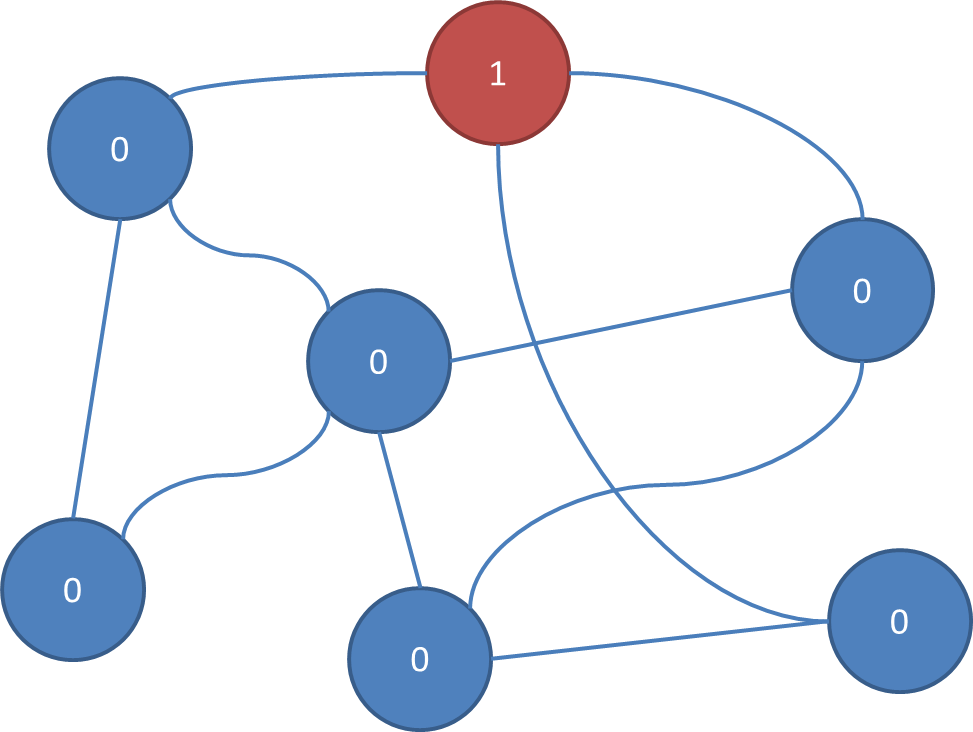
\includegraphics[width=6cm]{qwd_part/1.png}<3>}}}
			\only{\centering{{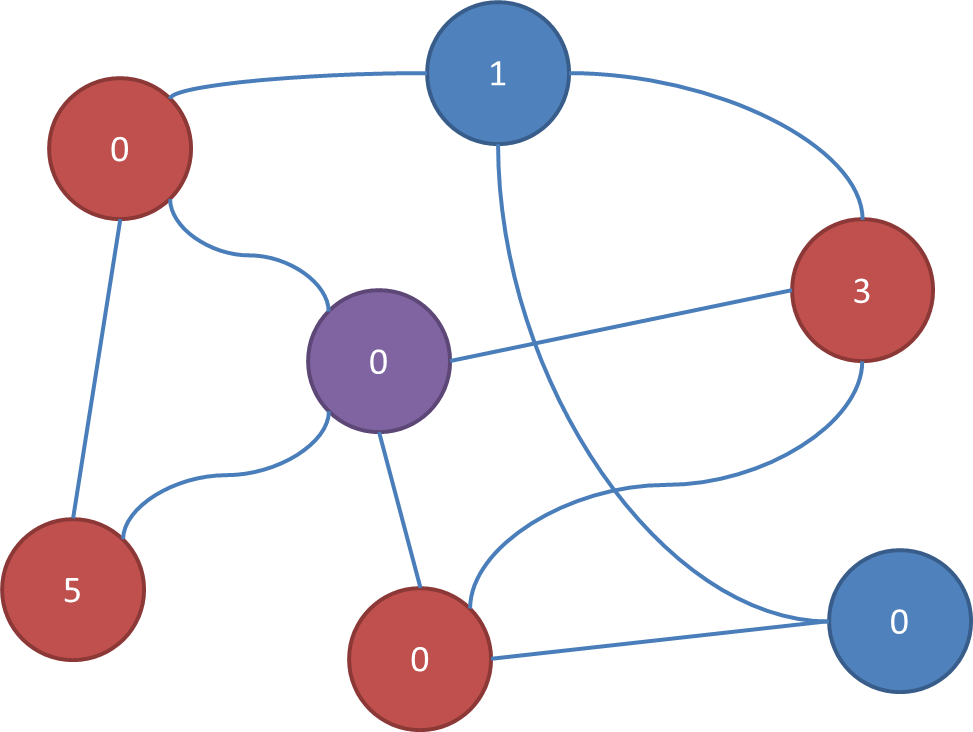
\includegraphics[width=6cm]{qwd_part/6.png}<4>}}}
		\end{columns}
	\end{frame}
	\begin{frame}[c]\frametitle{Naive Approach 2}
		\begin{columns}
			\column{4cm}
			\begin{itemize}
				\item<1-> store the sum $s[x]$
				\item<2-> $O(n)$ space
				\item<3-> $O(n)$ time for add
				\item<6-> $O(1)$ time for query
			\end{itemize}
			\column{6cm}
			\only{\centering{{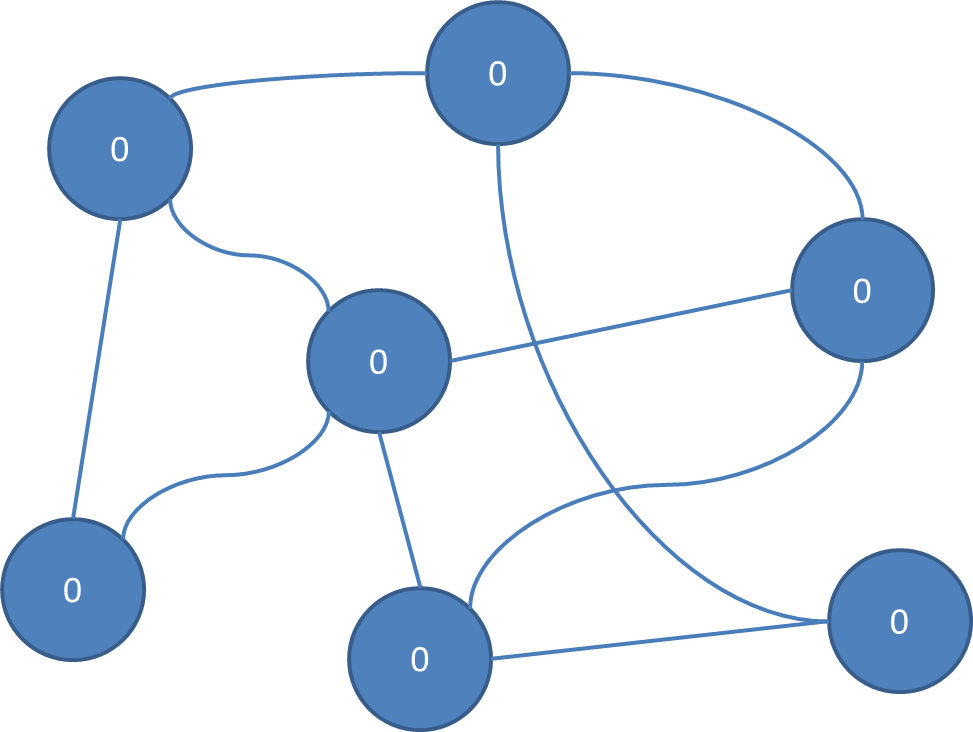
\includegraphics[width=6cm]{qwd_part/0.png}<1-2>}}}
			\only{\centering{{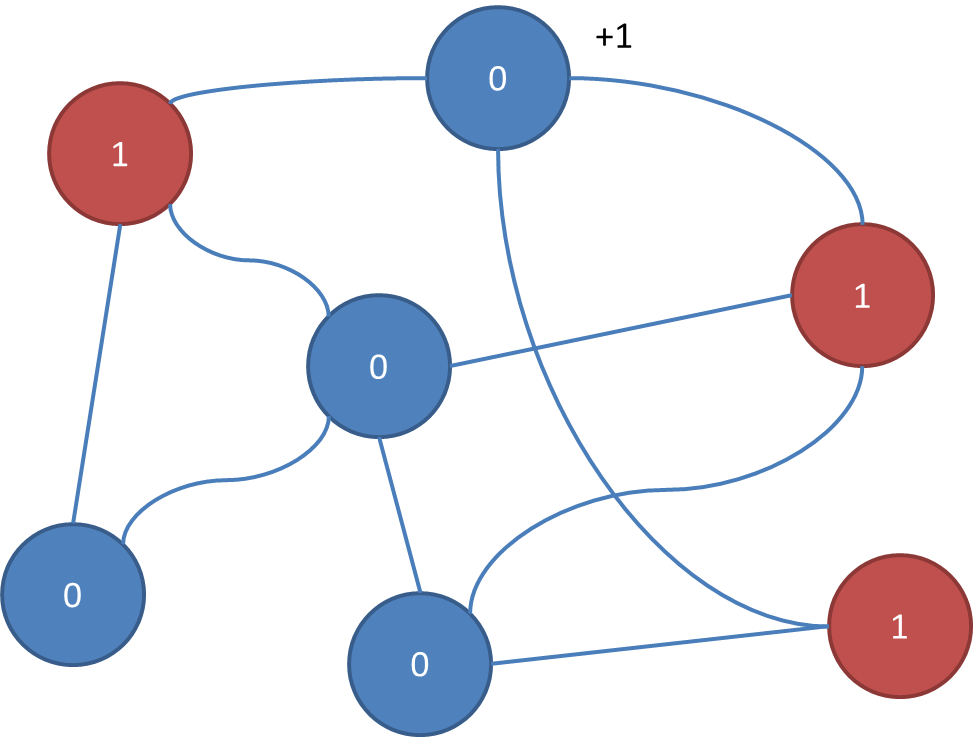
\includegraphics[width=6cm]{qwd_part/8.png}<3>}}}
			\only{\centering{{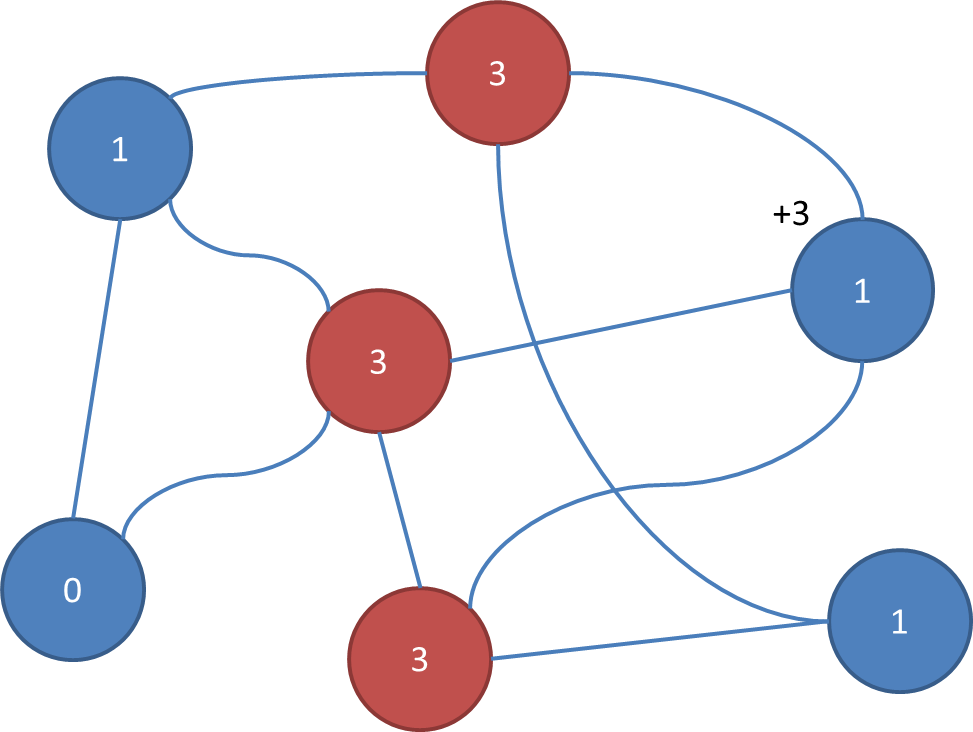
\includegraphics[width=6cm]{qwd_part/9.png}<4>}}}
			\only{\centering{{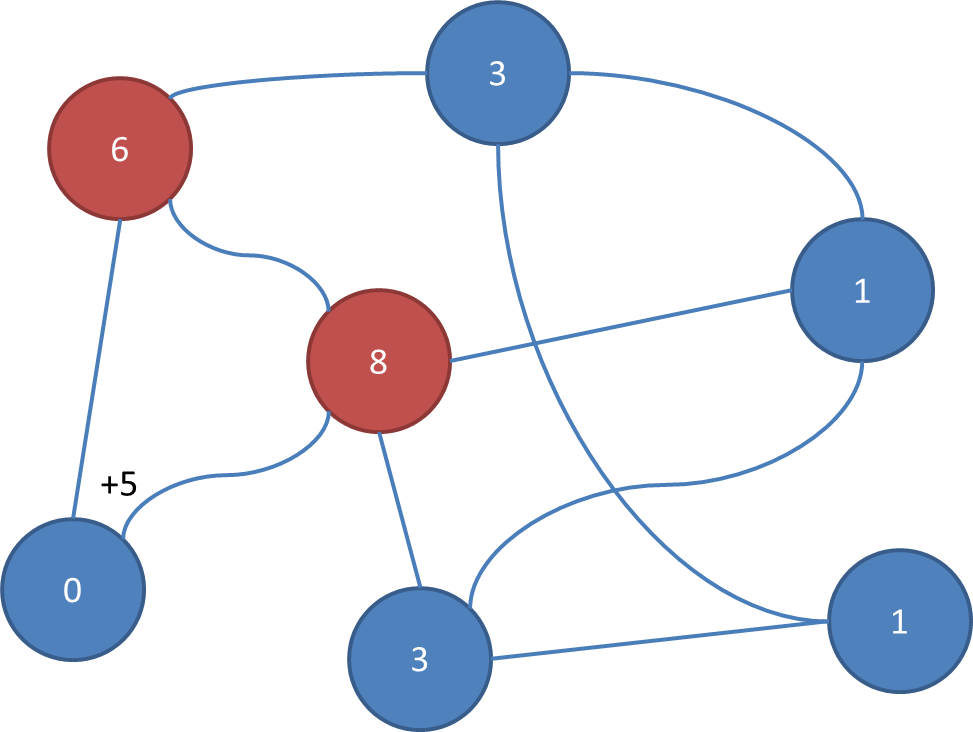
\includegraphics[width=6cm]{qwd_part/10.png}<5>}}}
			\only{\centering{{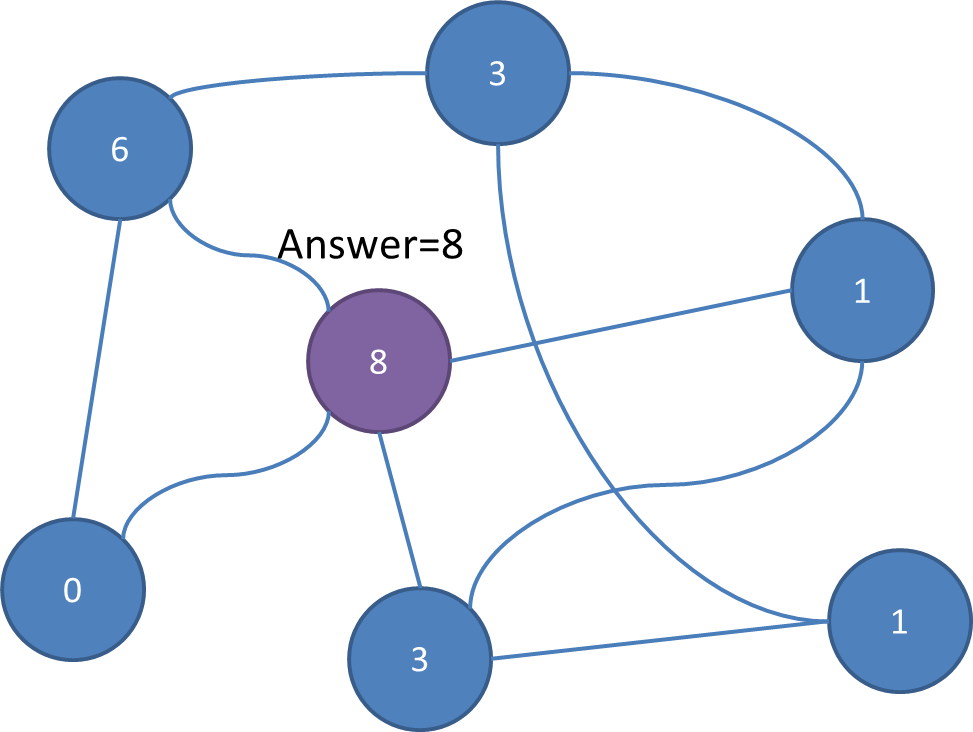
\includegraphics[width=6cm]{qwd_part/11.png}<6>}}}
		\end{columns}
	\end{frame}
	\begin{frame}[c]\frametitle{Observation}
		\begin{columns}
			\column{7cm}
			\beamerdefaultoverlayspecification{<+->}
			\begin{itemize}
				\item bad when large $deg(x)$
				\item "heavy" when $deg(x)>B$
			\end{itemize}
			\column{3cm}
			\only{\centering{{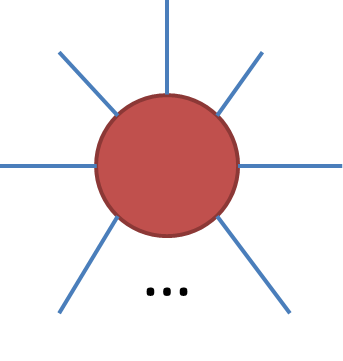
\includegraphics[width=2cm]{qwd_part/19.png}<1>}}}
			\only{\centering{{
\includegraphics[width=3cm]{qwd_part/20.png}<2>}}}
		\end{columns}
	\end{frame}
	\begin{frame}[c]\frametitle{Heavy-Light Divide}
		\only{\centering{{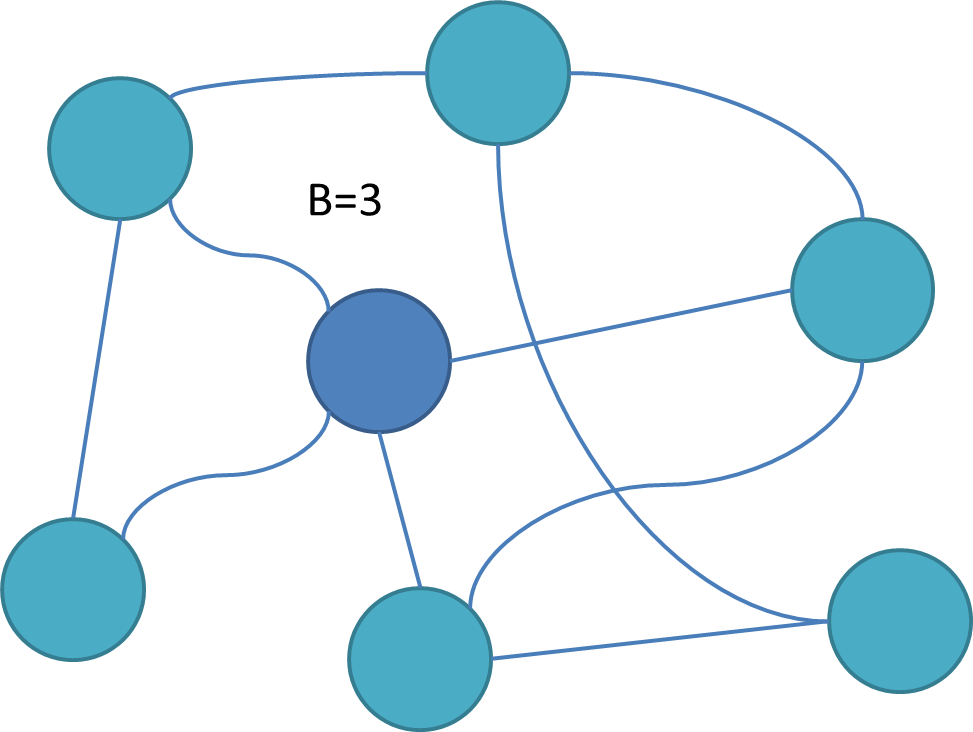
\includegraphics[width=8cm]{qwd_part/13.png}<1>}}}
		\only{\centering{{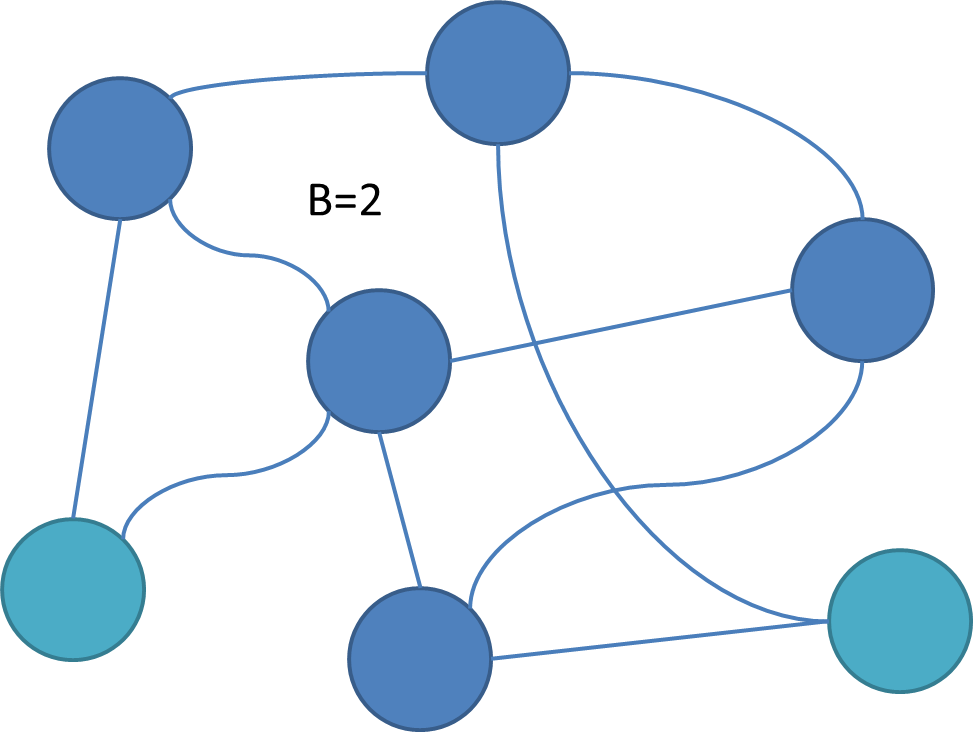
\includegraphics[width=8cm]{qwd_part/12.png}<2>}}}
	\end{frame}
	\begin{frame}[c]\frametitle{Combined Approach}
		\begin{columns}
			\column{5cm}
			\begin{itemize}
				\item<1-> $s[x]=\sum v[heavy\ neighbors]+\sum v[light\ neighbors]$
				\item<2-> for $\sum v[heavy\ neighbors]$ use approach 1
				\item<2-> for $\sum v[light\ neighbors]$ use approach 2
			\end{itemize}
			\column{5cm}
			\only{\centering{{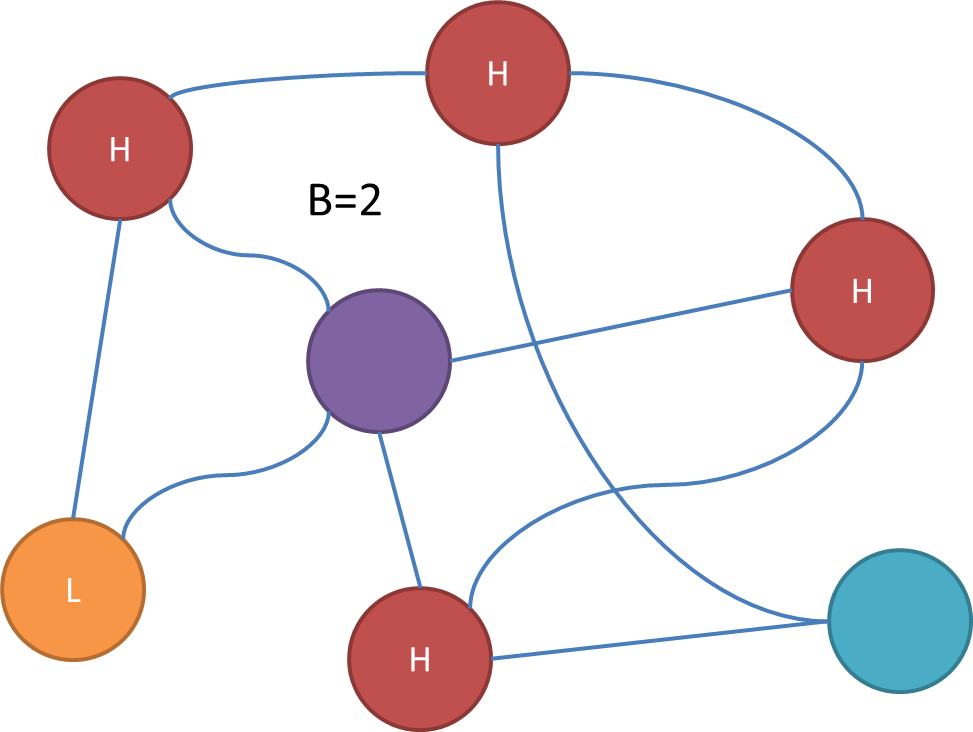
\includegraphics[width=5cm]{qwd_part/21.png}}}}
		\end{columns}
	\end{frame}
	\begin{frame}[c]\frametitle{$Add(u,x)$ details}
		\begin{columns}
			\column{4cm}
			\begin{itemize}
				\item<1-> if $u$ is heavy, $vh[u]\leftarrow vh[u]+x$
				\item<3-> if $u$ is light, $sl[v]\leftarrow sl[v]+x$, $u,v$ are neighbors
				\item<4-> $O(1)$ time for heavy
				\item<5-> $O(B)$ time for light
			\end{itemize}
			\column{6cm}
			\only{\centering{{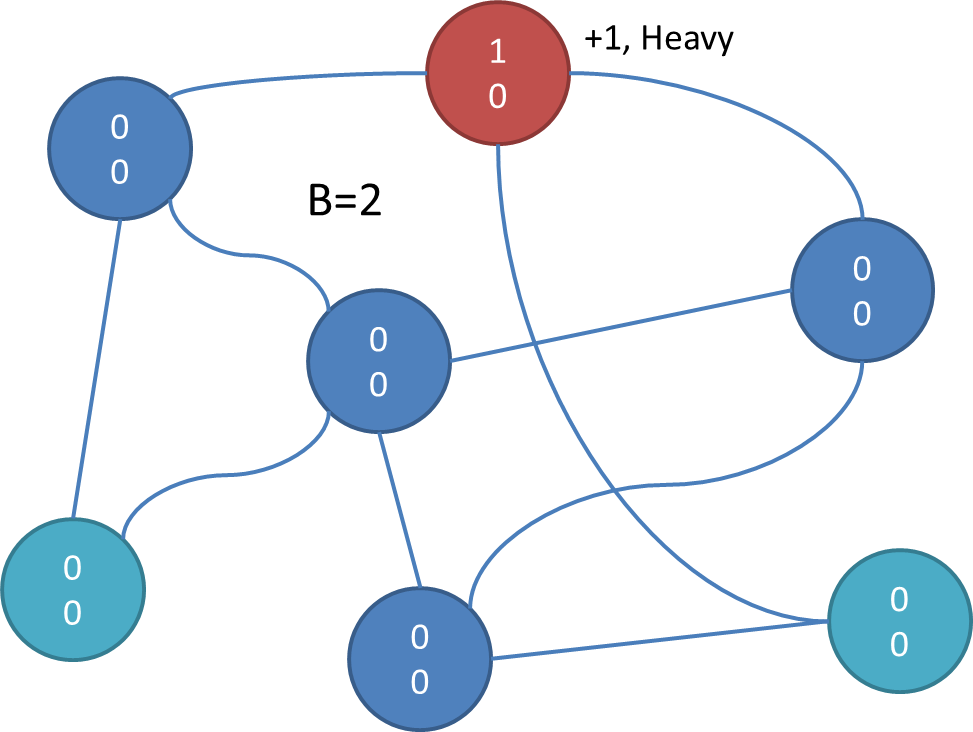
\includegraphics[width=6cm]{qwd_part/15.png}<1>}}}
			\only{\centering{{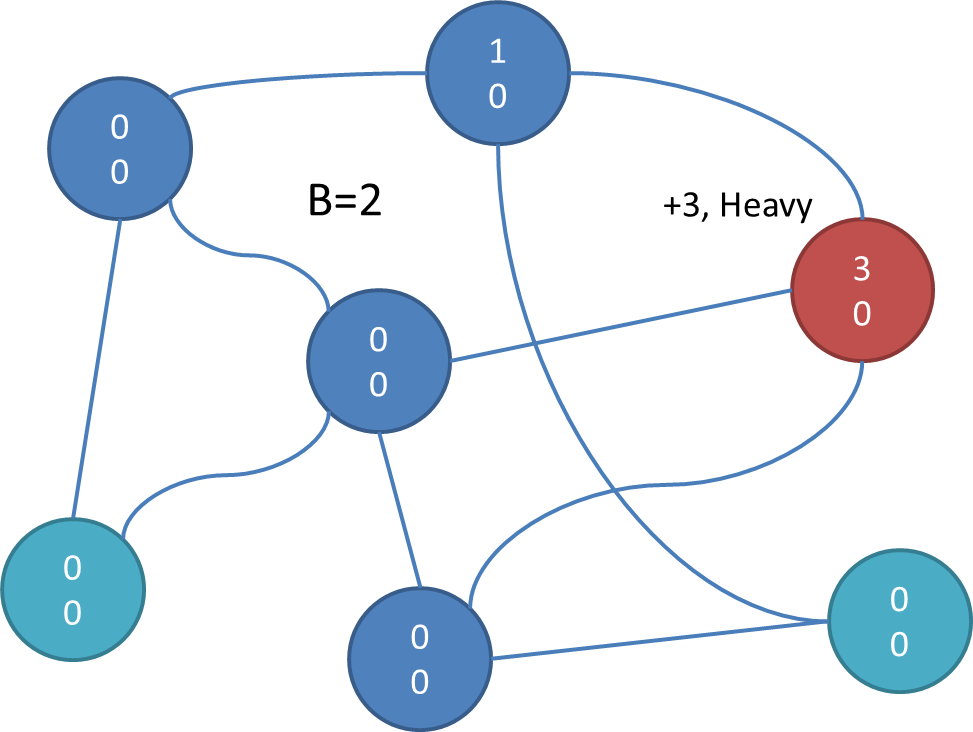
\includegraphics[width=6cm]{qwd_part/16.png}<2>}}}
			\only{\centering{{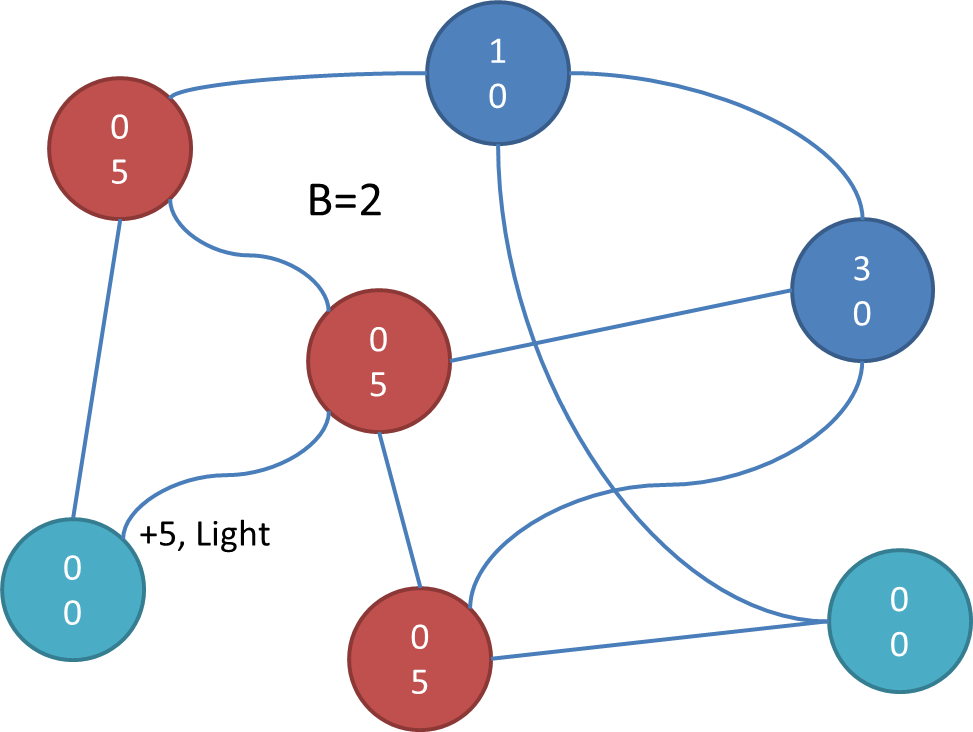
\includegraphics[width=6cm]{qwd_part/17.png}<3>}}}
			\only{\centering{{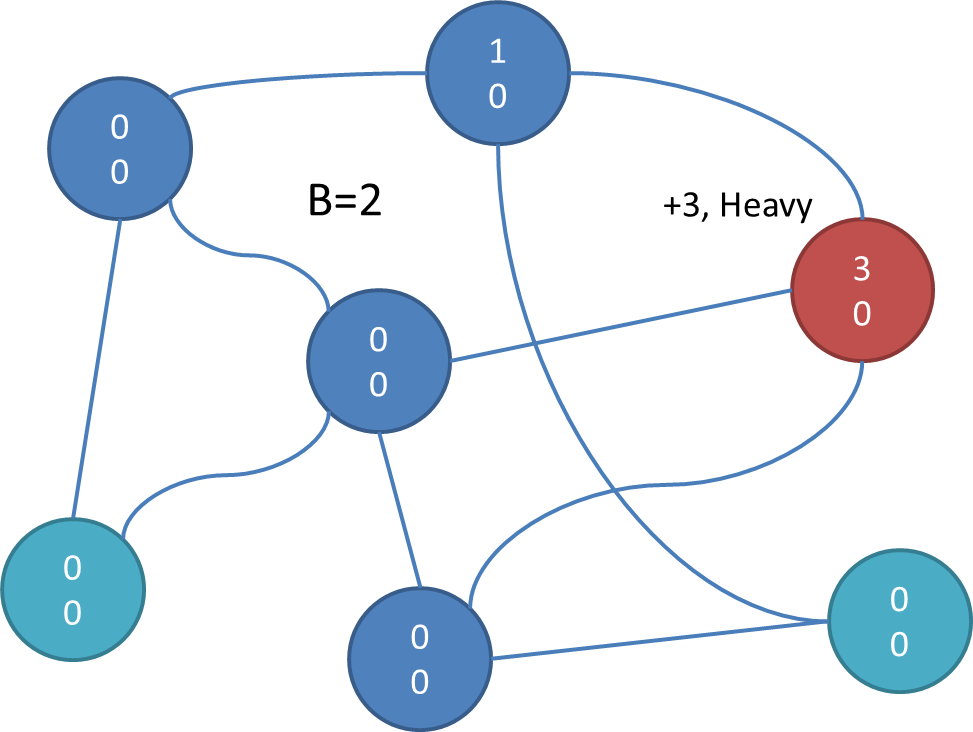
\includegraphics[width=6cm]{qwd_part/16.png}<4>}}}
			\only{\centering{{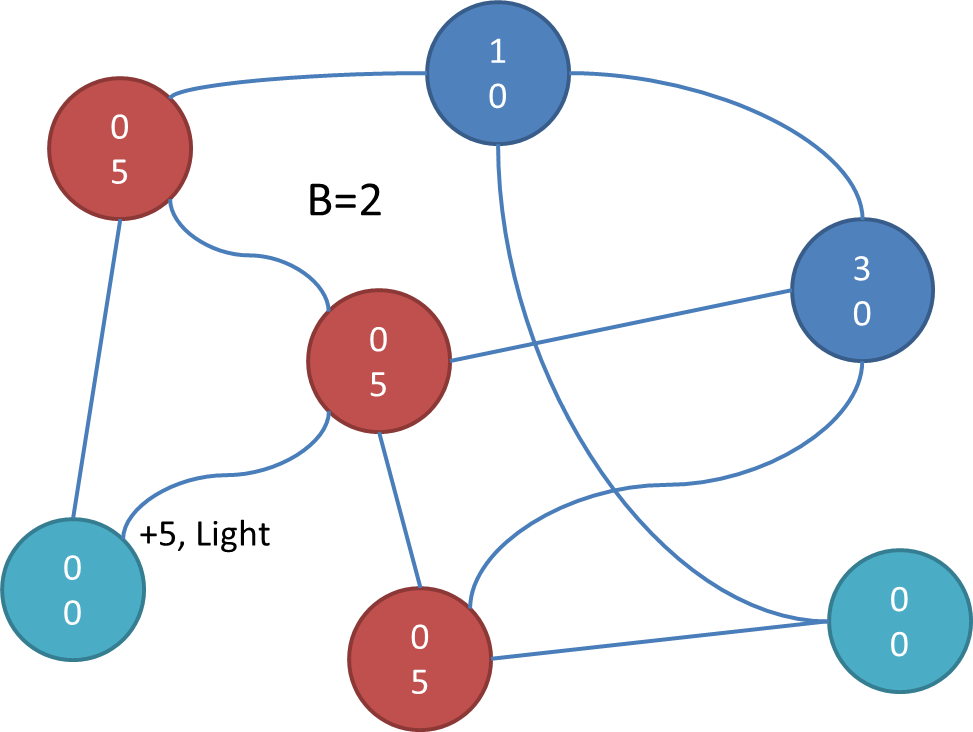
\includegraphics[width=6cm]{qwd_part/17.png}<5>}}}
		\end{columns}
	\end{frame}
	\begin{frame}[c]\frametitle{$Query(x)$ details}
		\begin{columns}
			\column{5.4cm}
			\begin{itemize}
				%\item $s[x]=\sum v[heavy\ neighbors]+\sum v[light\ neighbors]$
				\item<1-> $\sum v[heavy\ neighbors]=\sum_{y\ is\ heavy\  neighbor}vh[y]$
				\item<2-> $\sum v[light\ neighbors]=sl[x]$
				%\item $adj(x,y)=\left\{
				%	\begin{aligned}
				%	&1& x, y\ are\ neighbors \\
				%	&0& otherwise
				%	\end{aligned}
				%	\right. $
				\item<4-> $O(1+cnt\_heavy)$ time
				\item<5-> $cnt\_heavy \cdot B\leq 2m=O(n)$
				\item<6-> $O(n/B)$ time
			\end{itemize}
			\column{5cm}
			\only{\centering{{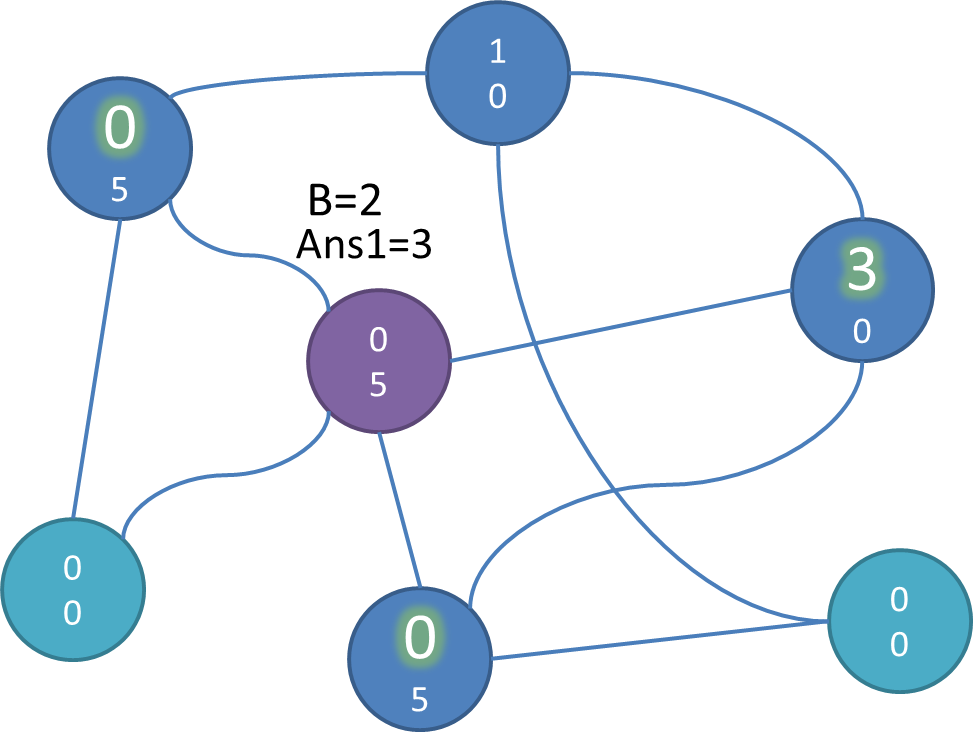
\includegraphics[width=5cm]{qwd_part/22.png}<1>}}}
			\only{\centering{{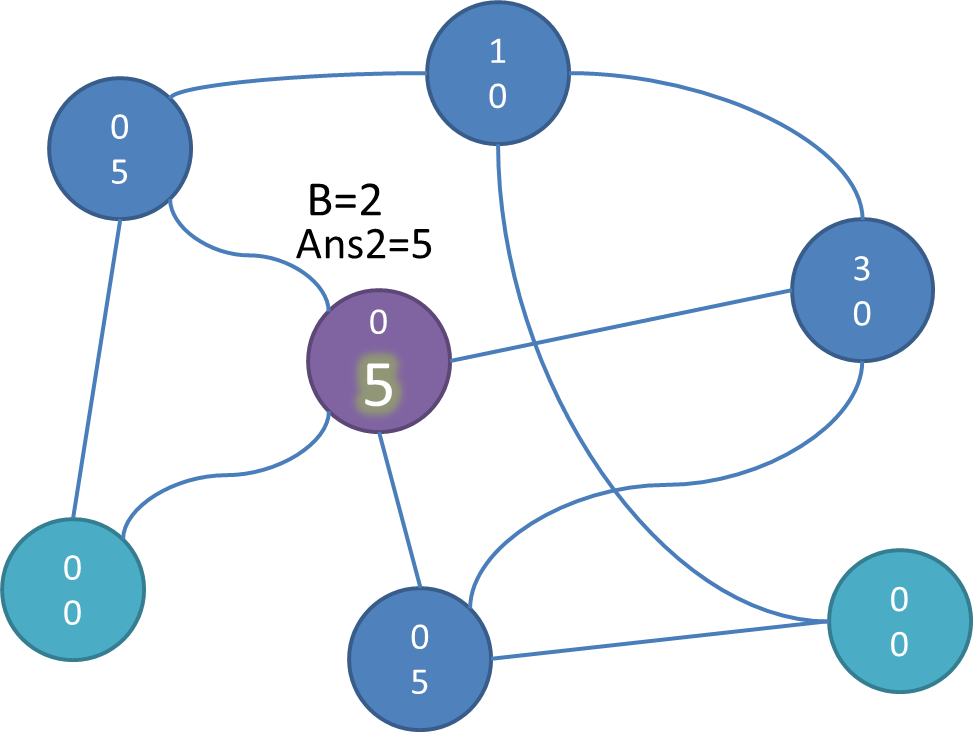
\includegraphics[width=5cm]{qwd_part/23.png}<2>}}}
			\only{\centering{{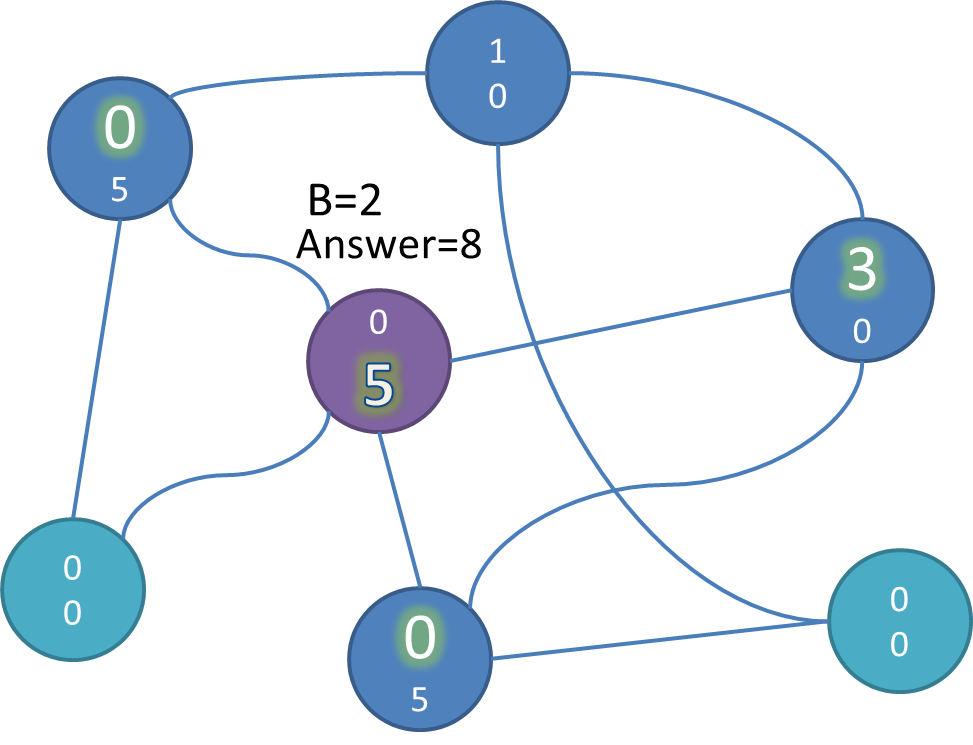
\includegraphics[width=5cm]{qwd_part/18.png}<3->}}}
		\end{columns}
	\end{frame}
	\begin{frame}[c]\frametitle{Balance}
		\beamerdefaultoverlayspecification{<+->}
		\begin{itemize}
			\item $O(n)$ space
			\item $O(B)$ time for add
			\item $O(n/B)$ time for query
			\item make $B=\sqrt{n}$
			\item $O(\sqrt{n})$ for each operation
		\end{itemize}
	\end{frame}
